
\section{Demonstration}
\label{sec:demonstration}

Figure~\ref{fig:workflow} presents the branch-separated computational
workflow. Shuffle/permutation controls define stochastic empirical control
distributions. Circular-shift controls instead use exhaustive nontrivial
radial offsets to define exact circular-shift randomization distributions.

\begin{figure}[htbp]
  \centering
  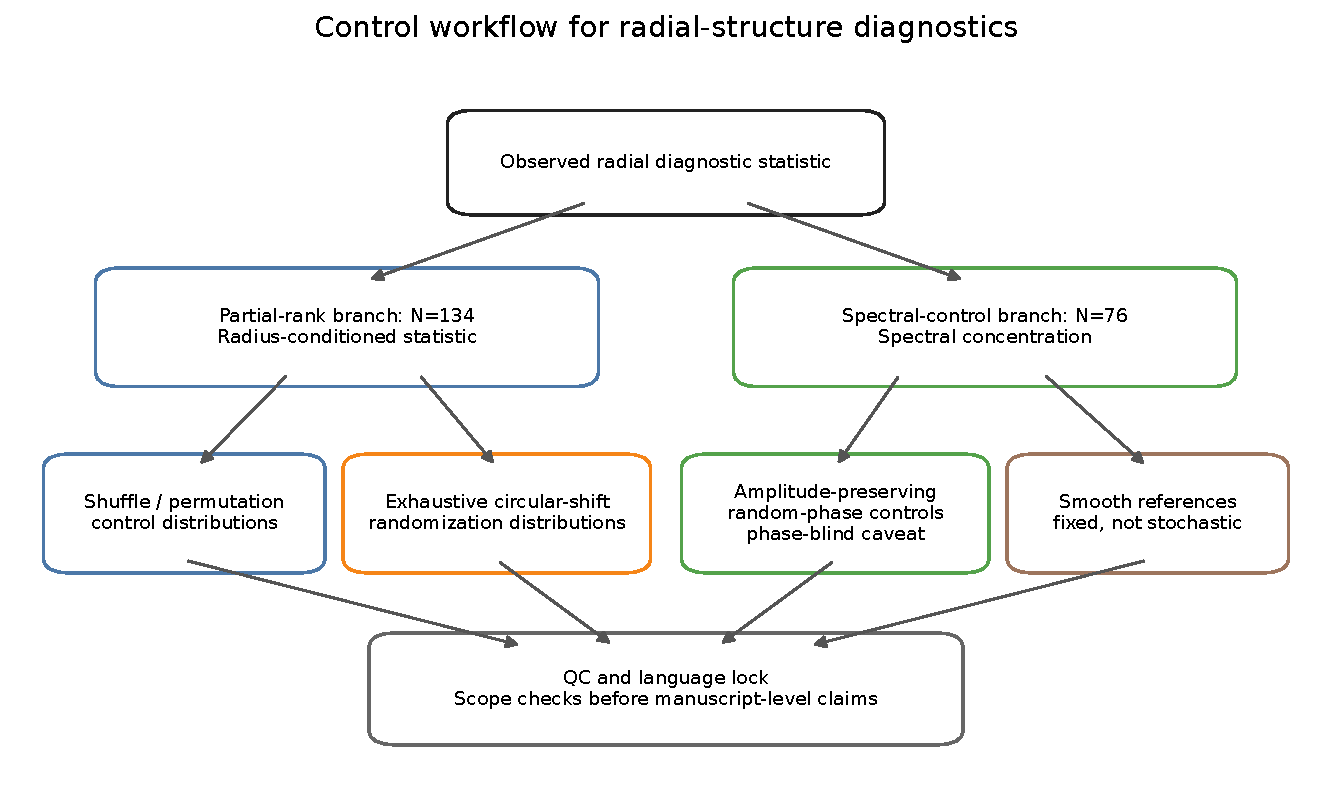
\includegraphics[width=\linewidth]{../figures/figure1_workflow_control_validation_rev1.pdf}
  \caption{Control workflow for radial-structure diagnostics. The workflow
  separates the $N=134$ partial-rank branch from the $N=76$ spectral-control
  branch. Shuffle/permutation controls form stochastic empirical control
  distributions, whereas circular-shift controls use exhaustive nontrivial
  radial offsets to define exact circular-shift randomization distributions.
  Amplitude-preserving random-phase controls carry a phase-blind/by-construction
  caveat. Smooth profiles are fixed references, not stochastic controls.}
  \label{fig:workflow}
\end{figure}

For the $N=134$ partial-rank branch, the observed absolute statistic has
median $\simeq0.509$ (IQR $0.280$--$0.773$). Per-galaxy shuffle-control
medians have median $\simeq0.182$ (IQR $0.135$--$0.232$), while exact
circular-shift medians have median $\simeq0.532$ (IQR $0.340$--$0.649$).
Across galaxies, the corresponding empirical p-values have medians
$\simeq0.026$ and $0.500$, respectively. These summaries are not
pooled-across-galaxy p-values.

For the separate $N=76$ spectral branch, residual and radial-template spectral
concentrations have medians $\simeq0.676$ (IQR $0.589$--$0.755$) and
$\simeq0.754$ (IQR $0.663$--$0.817$), respectively. Random-phase control
medians are identical at displayed precision by construction. The
exponential, linear, and quadratic fixed-reference values are approximately
$0.548$, $0.553$, and $0.570$.

\begin{figure}[htbp]
  \centering
  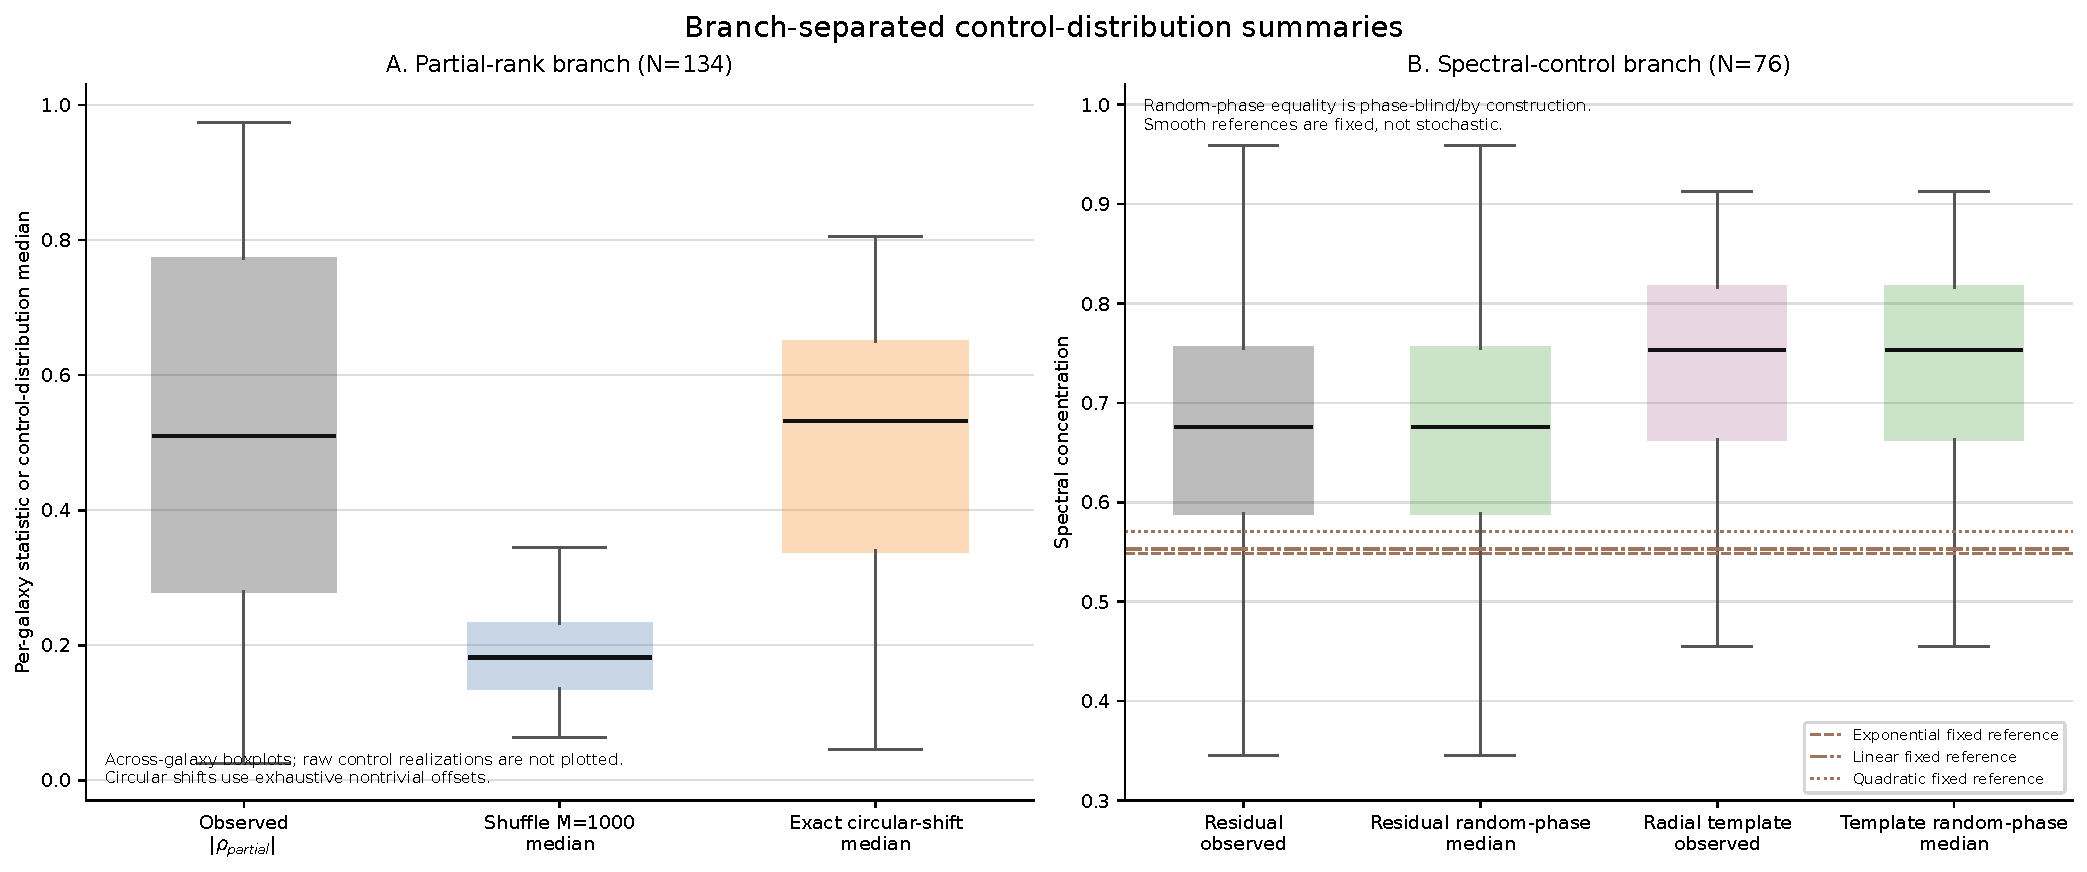
\includegraphics[width=\linewidth]{../figures/figure2_control_distribution_comparison_rev1.pdf}
  \caption{Branch-separated control-distribution summaries. Panel A shows the
  $N=134$ partial-rank branch and per-galaxy medians from the $M=1000$
  shuffle empirical control distributions and exhaustive circular-shift
  randomization distributions. Panel B separately shows the $N=76$
  spectral-control branch, random-phase control medians, and smooth-profile
  fixed references. Panels summarize each per-galaxy control distribution by
  its median; empirical percentiles and p-values remain in the production
  summary table, and the full raw realizations are not plotted. Fixed
  references are not stochastic controls.}
  \label{fig:control-summaries}
\end{figure}

For both spectral targets, per-galaxy mid-rank empirical percentiles are
$0.500$ and doubled equal-tail quantities are $1.000$. This follows from
amplitude preservation and the definition of spectral concentration.

\begin{figure}[htbp]
  \centering
  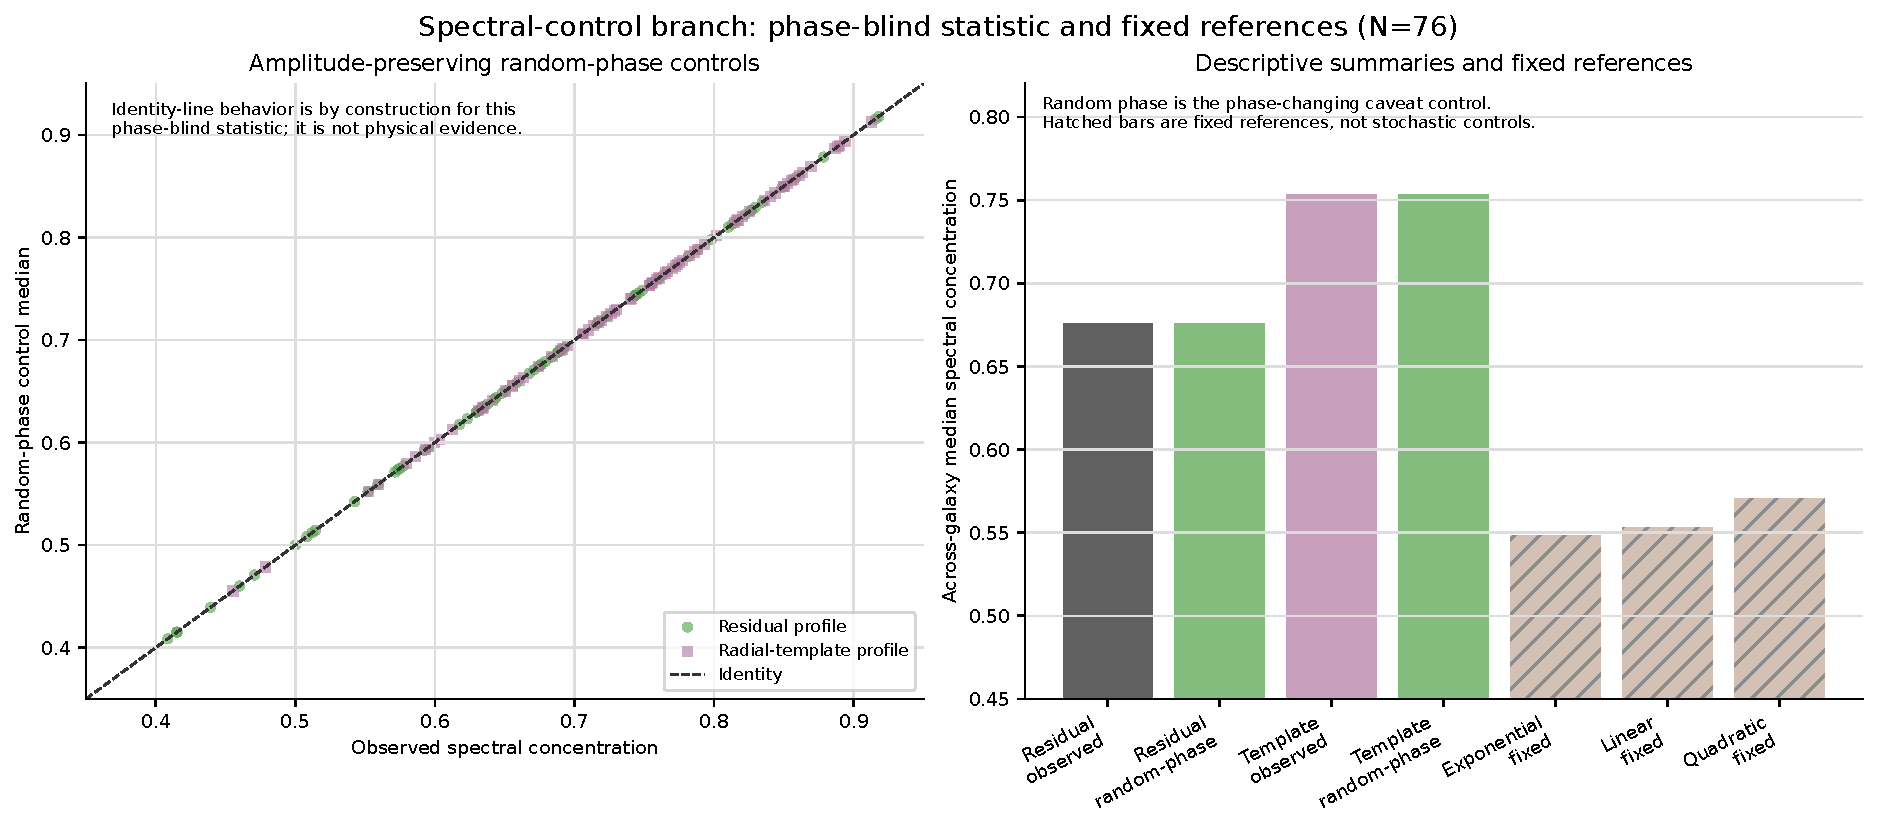
\includegraphics[width=\linewidth]{../figures/figure3_spectral_phase_control_caveat_rev1.pdf}
  \caption{Phase-blind spectral-concentration caveat and fixed references
  ($N=76$). Panel A compares observed spectral concentration with per-galaxy
  medians from amplitude-preserving random-phase controls. Identity-line
  behavior is by construction for the phase-blind statistic and is not
  independent evidence about the profiles. Panel B shows descriptive
  across-galaxy medians; smooth profiles are fixed references, not stochastic
  controls.}
  \label{fig:spectral-caveat}
\end{figure}
